% Notes: docs/exhibits.md#fig_draft_final_gap
\begin{figure}[!ht]
  \centering
  \setlength{\tabcolsep}{1pt}%
  % All views are the same 1:1 frame (1080 bp source);
  % the zoom box keeps the source region x 162--702, y 695--875 bp from the bottom.
  % TODO: Replace the middle panel and its crop with the actual draft image
  % produced by lightweight multi-frame composition. Both temporarily reuse
  % fig_draft_final_gap_final.jpg; the caption explicitly marks this placeholder.
  \begin{tabular}{@{}ccc@{}}
    \begin{tikzpicture}
      \node[inner sep=0, anchor=south west] (im) at (0,0)
        {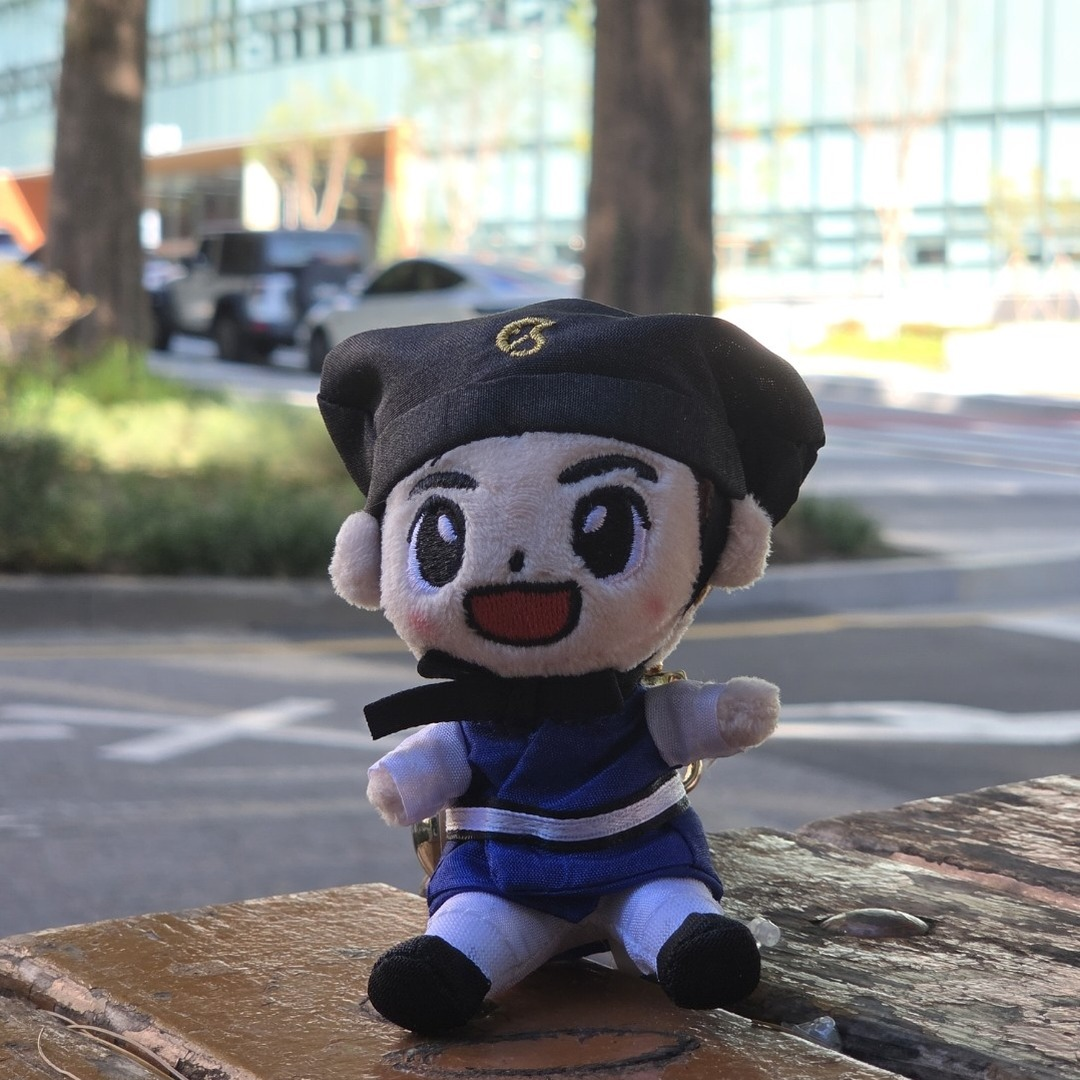
\includegraphics[width=0.325\columnwidth]{figures/fig_draft_final_gap_draft.jpg}};
      \begin{scope}[x={(im.south east)}, y={(im.north west)}]
        \draw[orange, line width=0.8pt] (0.15,0.6435) rectangle (0.65,0.8102);
      \end{scope}
    \end{tikzpicture} &
    \begin{tikzpicture}
      \node[inner sep=0, anchor=south west] (im) at (0,0)
        {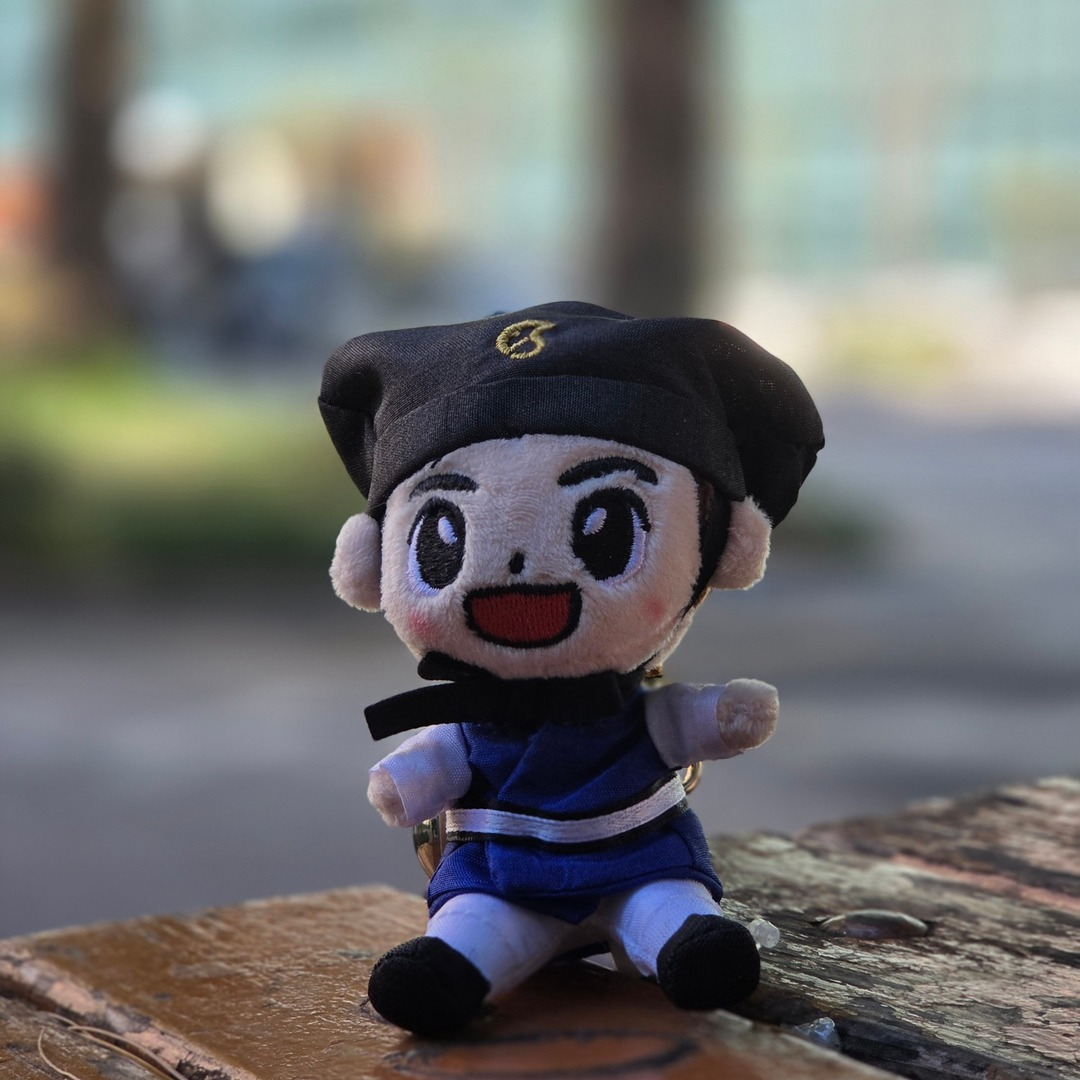
\includegraphics[width=0.325\columnwidth]{figures/fig_draft_final_gap_final.jpg}};
      \begin{scope}[x={(im.south east)}, y={(im.north west)}]
        \draw[orange, line width=0.8pt] (0.15,0.6435) rectangle (0.65,0.8102);
      \end{scope}
    \end{tikzpicture} &
    \begin{tikzpicture}
      \node[inner sep=0, anchor=south west] (im) at (0,0)
        {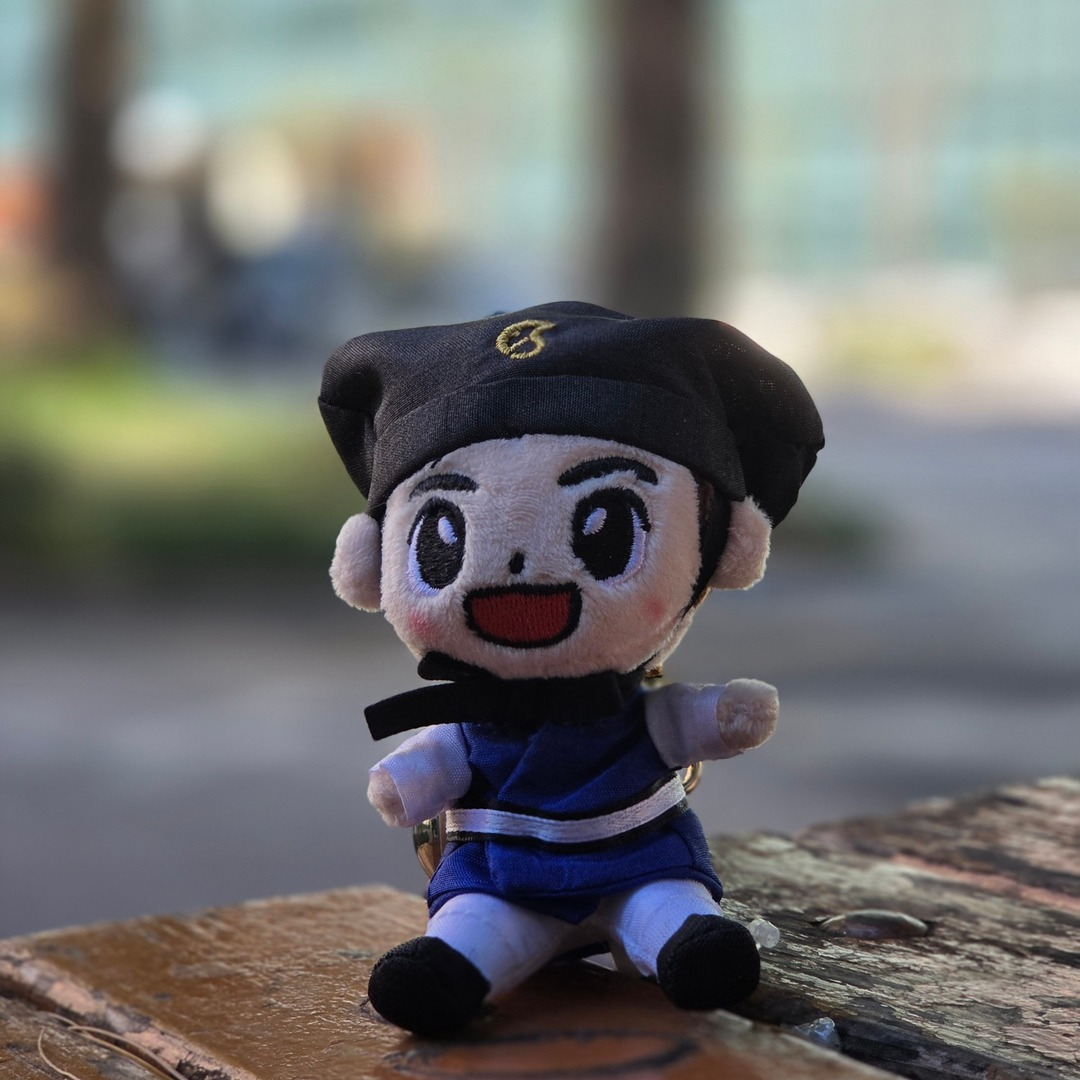
\includegraphics[width=0.325\columnwidth]{figures/fig_draft_final_gap_final.jpg}};
      \begin{scope}[x={(im.south east)}, y={(im.north west)}]
        \draw[orange, line width=0.8pt] (0.15,0.6435) rectangle (0.65,0.8102);
      \end{scope}
    \end{tikzpicture} \tabularnewline[1pt]
    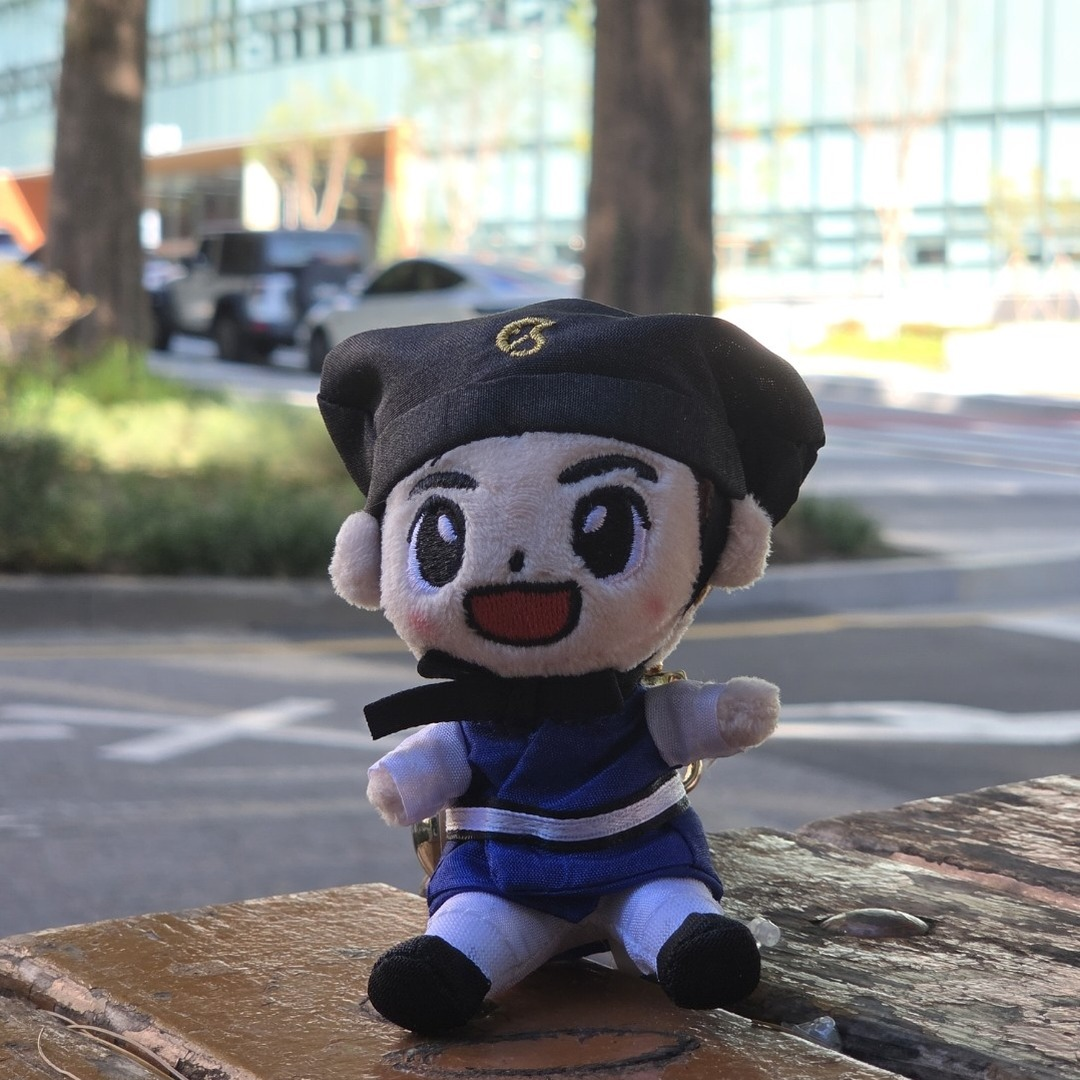
\includegraphics[width=0.325\columnwidth, trim=162 695 378 205, clip]{figures/fig_draft_final_gap_draft.jpg} &
    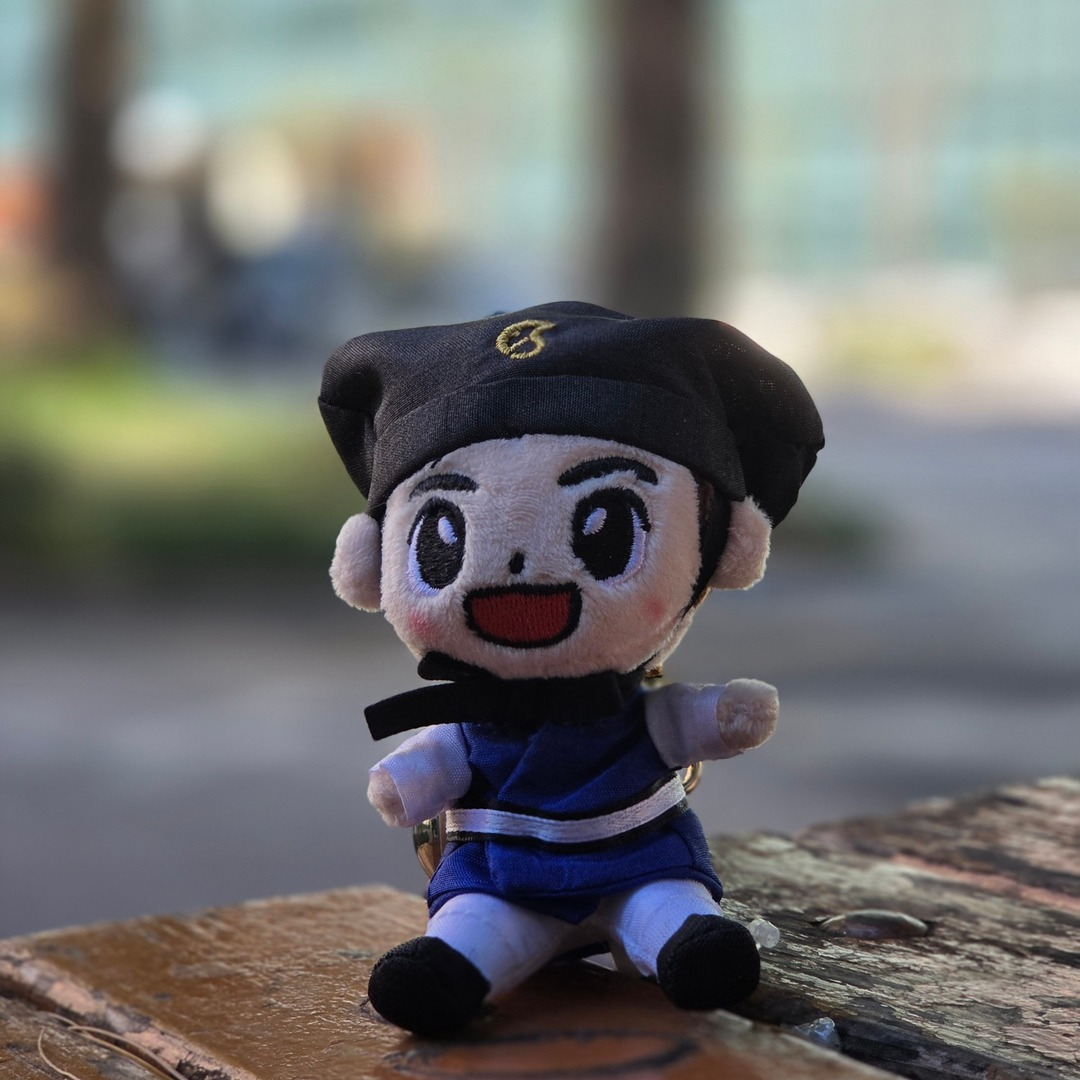
\includegraphics[width=0.325\columnwidth, trim=162 695 378 205, clip]{figures/fig_draft_final_gap_final.jpg} &
    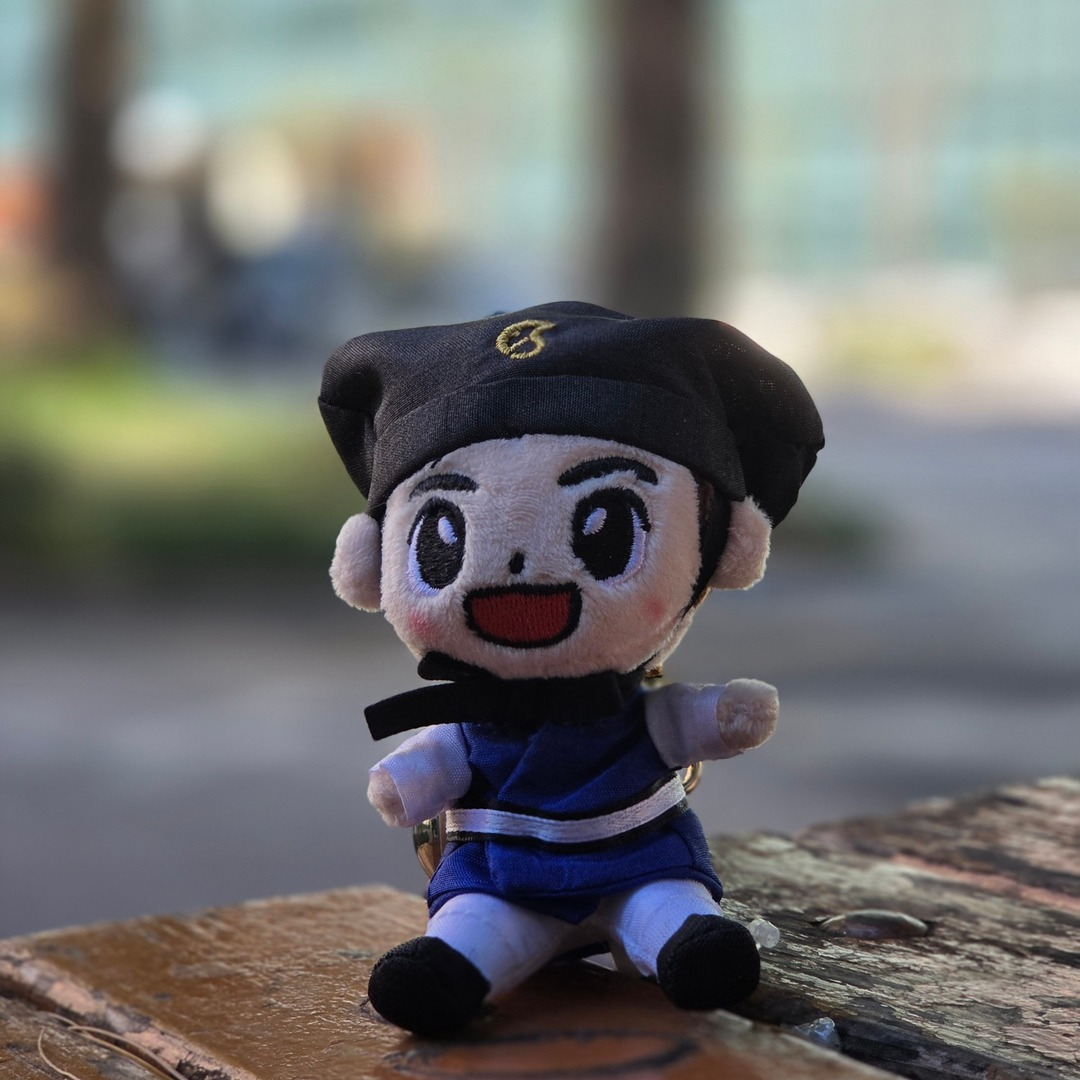
\includegraphics[width=0.325\columnwidth, trim=162 695 378 205, clip]{figures/fig_draft_final_gap_final.jpg}
    \tabularnewline[2pt]
    \parbox[t]{0.325\columnwidth}{\centering\scriptsize (a) Draft image} &
    \makebox[0.325\columnwidth][c]{%
      \parbox[t]{0.41\columnwidth}{\centering\scriptsize
        (b) Draft image with \\lightweight multi-frame composition}} &
    \parbox[t]{0.325\columnwidth}{\centering\scriptsize (c) Final image}
  \end{tabular}
  \caption{Draft--final visual differences in Portrait mode.}
  \label{fig:draft-final-gap}
\end{figure}
